% Ontogenic Learning preprint — living draft. Build: latexmk -pdf main.tex (or make).
% Convention: every number in a table traces to a JSONL in ../results/; update tables
% ONLY from regenerated logs, and re-run figs/make_figs.py when results change.
\documentclass[11pt]{article}
\usepackage[margin=1.05in]{geometry}
\usepackage{amsmath,amssymb}
\usepackage{booktabs}
\usepackage{graphicx}
\usepackage{microtype}
\usepackage{xcolor}
\usepackage[colorlinks=true,linkcolor=blue!60!black,citecolor=blue!60!black,urlcolor=blue!60!black]{hyperref}
\usepackage[numbers,sort&compress]{natbib}

\newcommand{\todo}[1]{\textcolor{red!70!black}{[TODO: #1]}}
\newcommand{\gate}[1]{\textsf{#1}}

\title{Surprise-Gated Two-Speed Learning on a Multiply-Free Substrate:\\
A Retention--Plasticity--Energy Dial for Always-On Language Models}

\author{%
  \todo{author list / affiliation / order}\\
  \small NYU OLab $\cdot$ the TikiTorch project\\
  \small \texttt{https://github.com/nyuolab/tikitorch} (\texttt{ontogenic\_learner/})}
\date{Working draft --- \today\ --- v0.1 (G1--G1.2 results in; G1b/G2/G3 pending)}

\begin{document}
\maketitle

\begin{abstract}
Deployed language models are frozen artifacts: learning happens in a separate batch phase, on
different hardware, and adaptation is rationed through fine-tuning cycles that forget. We study
the opposite regime --- \emph{ontogenic learning}: a model that keeps learning, in place, from a
strictly sequential non-i.i.d.\ experience stream, under a matched update budget. We introduce a
\emph{two-speed learner}: fast plastic updates are applied only when a surprise gate
$z(\varepsilon)>\tau$ fires on the stream (an error-gated, neuromodulatory-style plasticity
signal), while slow low-learning-rate consolidation passes replay a surprise-weighted reservoir
(``sleep''). On a character-LM substrate with multiply-free ($\pm2^k$ dyadic) forward weights
--- chosen because the same learner maps kick-for-kick onto an FPGA training fabric with
per-kick plasticity knobs and bit-exact update audit --- the two-speed learner
\textbf{Pareto-dominates matched-budget rehearsal backprop} across a Wikipedia
$\rightarrow$ Shakespeare $\rightarrow$ technical-docs $\rightarrow$ source-code stream:
$33\%$ less forgetting at $98\%$ plasticity, replicated over strengthened controls
(domain-balanced and $50\%$-replay rehearsal). The gate threshold $\tau$ acts as a single
scalar dial trading retention, plasticity, and energy: at $\tau{=}1.5$ the learner updates on
${\sim}7\%$ of stream batches, spends $40\%$ of the update budget, and retains prior domains
essentially without forgetting ($+0.03$ bpc) at $80\%$ plasticity. All experiments are
pre-registered with kill criteria, seeds and event logs are released, and we report an honesty
ledger including what the method does \emph{not} yet show (rule-level advantages of iterative
predictive coding remain unproven at this scale). \todo{revise abstract as G2/G3 land}
\end{abstract}

\section{Introduction}\label{sec:intro}

The scaling era optimized parameters$\times$tokens on static corpora. That axis belongs to
synchronous backprop on dense accelerators and, we argue, always will; we make no claim against
it. A different axis is opening: \emph{experience$\times$time} --- systems that learn
continuously from their own deployment streams
\citep{silver2025era,sutton2024loss}. Nothing shipped today occupies it: test-time-training
architectures reset their fast weights per session \citep{behrouz2025titans}, and production
``fleet learning'' loops centralize data while weights train in the datacenter. Meanwhile the
blockers are now quantified: catastrophic forgetting under sequential fine-tuning, and loss of
plasticity, which scale delays but does not repair \citep{dohare2024loss}.

We take the biological answer seriously as an engineering hypothesis, not a slogan: learning
gated by surprise (neuromodulatory tone), two timescales of consolidation (wake/sleep,
complementary learning systems), local credit assignment, and a strict energy budget. We
operationalize these as a minimal, fully-measurable learner (\S\ref{sec:method}), pre-register
the decisive comparison against matched-budget rehearsal backprop, and report the result
(\S\ref{sec:results}).

Contributions: \textbf{(1)} the two-speed learner --- $\varepsilon$-gated fast cascade kicks +
surprise-weighted reservoir sleep --- which Pareto-dominates strengthened rehearsal controls on
a sequential domain stream at matched update budget; \textbf{(2)} the $\tau$ dial: a single
scalar exposing a smooth retention--plasticity--energy control surface, reaching near-zero
forgetting at $40\%$ energy; \textbf{(3)} a substrate mapping: every learner primitive
(gate, kick, sleep, replay) corresponds one-to-one to per-kick host-staged knobs of a measured
FPGA training fabric with bit-exact update auditing, making the learner deployable where
GPUs cannot sit; \textbf{(4)} a pre-registered gate ladder with kill criteria and an honesty
ledger, including a logged negative.

\section{Related work}\label{sec:related}
\todo{expand each into a paragraph}
\textbf{Continual learning \& forgetting:} rehearsal/replay; LoRA forgetting trade
\citep{biderman2024lora}; sparse memory fine-tuning \citep{meta2025sparsemem} --- the strongest
SGD-family baseline for later gates. \textbf{Plasticity loss:} \citep{dohare2024loss} and
successors. \textbf{Test-time training / fast weights:} \citep{behrouz2025titans,
ttte2e2025} --- session-scoped, contrasted with persistent plasticity here.
\textbf{Low-communication distributed training:} DiLoCo \citep{douillard2023diloco} ---
replica-level locality on GPUs; our layer-level locality is complementary and is the fabric's
native regime. \textbf{Predictive coding:} equivalence of converged PC and backprop; $\mu$PC
depth scaling \citep{mupc2025}; prospective configuration \citep{song2024inferring};
associative/generative PC \citep{salvatori2021associative}. \textbf{Substrate:} the TikiTorch
multiply-free dyadic stack and the F2 training fabric \todo{cite internal reports/repo}.

\section{The two-speed learner}\label{sec:method}

\paragraph{Setting.} A model $f_\theta$ is deployed on a strictly sequential stream of batches
$b_1, b_2, \dots$ whose domain changes at unknown times, under a budget of $B$ applied updates
per domain segment. No i.i.d.\ reshuffling; evaluation is a transfer matrix over held-out
tails of every domain after every segment.

\paragraph{Surprise gate (wake).} A running estimate $(\mu,\sigma)$ of the batch loss yields a
z-scored surprise $z_t = (\ell_t-\mu)/\sigma$. A fast, plastic update (the \emph{cascade} step
--- gradient-checked equivalent to backprop on this stack) is applied only when $z_t > \tau$;
the batch is then inserted into a replay reservoir with priority $\max(z_t, 0.1)$. Boring data
causes no update at all --- this is where the energy budget is saved.

\paragraph{Sleep (consolidation).} Every $K$ stream batches, $S$ low-learning-rate updates are
taken on reservoir samples drawn proportionally to stored surprise. We ablate the sleep rule:
cascade (schedule-only) vs.\ iterative settled predictive coding (settle-then-local-update),
the regime in which PC differs from backprop.

\paragraph{Substrate and fabric mapping.} The model is a Bengio-style context char-LM on
DyadicPCNet (multiply-free $\pm2^k$ forward). On the F2 training fabric the learner is a host
policy over existing per-kick knobs: gate $\to$ \texttt{DO\_UP}, learning-rate schedule $\to$
\texttt{LRBITS}, accumulate/apply windows $\to$ \texttt{GZERO}; every applied update is
bit-exactly replayable at ${\sim}1\%$ overhead \todo{cite fabric measurements when G1b lands}.

\section{Pre-registered protocol}\label{sec:protocol}
Phylogeny: pretrain once on 5M chars of Wikipedia (\texttt{text8}); all arms start from the
identical checkpoint. Ontogeny: Shakespeare $\rightarrow$ technical documentation
$\rightarrow$ source code (frozen-base bpc 5.5/6.6/7.4 --- large ordered shifts); 1{,}500
stream batches and $B{=}600$ updates per domain; 3 seeds; all reservoirs seeded with the same
base-domain memories. Arms: frozen; sequential cascade (backprop); rehearsal at
$\{25\%,50\%\}\times\{\text{uniform},\text{domain-balanced}\}$; two-speed with
$\tau\in\{0,0.25,0.75,1.5\}$ and sleep-rule ablation. Go/No-Go (registered before running):
a two-speed arm must keep $\ge70\%$ of cascade plasticity \emph{and} Pareto-beat every
rehearsal control at matched budget. Full protocol: \texttt{PARADIGM.md} in the repository.

\section{Results}\label{sec:results}

\begin{table}[t]
\centering\small
\caption{G1/G1.2 (mean of 3 seeds; matched budget 600 updates/domain). Forgetting = bpc
regained on prior stream domains; plasticity = fraction of sequential-BP adaptation; energy =
applied updates. Source: \texttt{results/g1\_two\_speed/g1\_full\_g12.jsonl}.}
\label{tab:main}
\begin{tabular}{lccccc}
\toprule
arm & final avg bpc $\downarrow$ & forgetting $\downarrow$ & base drift $\downarrow$ &
plasticity $\uparrow$ & updates \\
\midrule
frozen                    & 6.548 & ---     & ---     & 0.00 & 0 \\
cascade (seq.\ BP)        & 3.529 & $+0.610$ & $+0.712$ & 1.00 & 1800 \\
rehearsal 25\%            & 3.615 & $+0.606$ & $+0.916$ & 0.97 & 1800 \\
rehearsal 25\% balanced   & 3.534 & $+0.510$ & $+0.795$ & 0.98 & 1800 \\
rehearsal 50\%            & 4.010 & $+0.834$ & $+1.316$ & 0.90 & 1800 \\
rehearsal 50\% balanced   & 3.823 & $+0.698$ & $+1.112$ & 0.93 & 1800 \\
\midrule
two-speed $\tau{=}0.00$   & \textbf{3.480} & $+0.311$ & $+0.591$ & 0.96 & 1755 \\
two-speed $\tau{=}0.25$   & 3.489 & $+0.442$ & $+0.573$ & \textbf{0.98} & 1746 \\
two-speed $\tau{=}0.75$   & 3.611 & $+0.253$ & $+0.546$ & 0.91 & 1212 \\
two-speed $\tau{=}1.50$   & 3.807 & $\mathbf{+0.030}$ & $+0.530$ & 0.80 & \textbf{717} \\
\bottomrule
\end{tabular}
\end{table}

\begin{figure}[t]
\centering
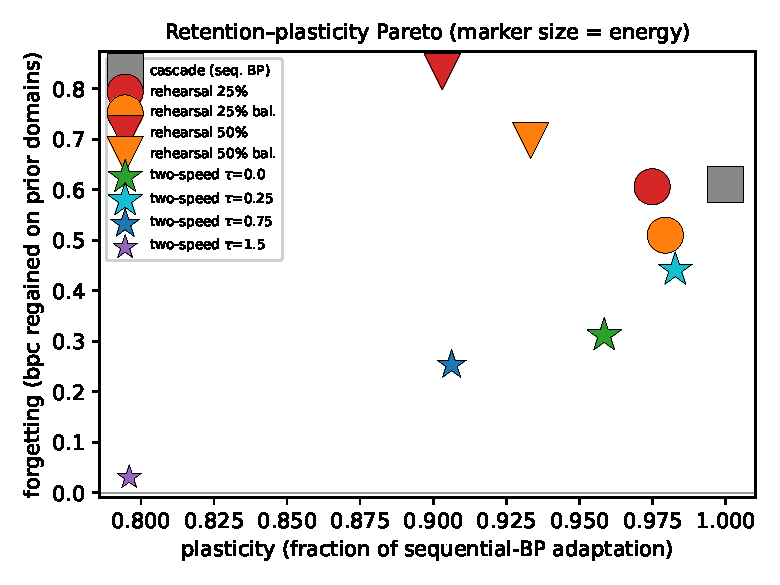
\includegraphics[width=.48\linewidth]{figs/pareto.pdf}\hfill
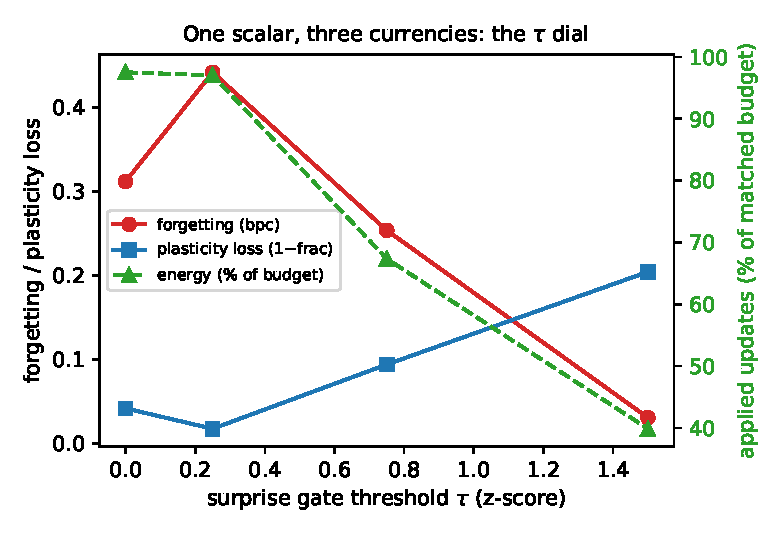
\includegraphics[width=.48\linewidth]{figs/dial.pdf}
\caption{\textbf{Left:} retention--plasticity plane; two-speed points (stars) dominate all
rehearsal controls (circles/triangles); marker size $\propto$ applied updates.
\textbf{Right:} the $\tau$ dial: one scalar trades forgetting, plasticity, and energy;
$\tau{=}1.5$ reaches near-zero forgetting at 40\% of the update budget.}
\label{fig:main}
\end{figure}

\paragraph{G1 --- the decisive comparison (GO).} Two-speed ($\tau{=}0.25$) Pareto-beats the
pre-registered rehearsal control: forgetting $+0.419$ vs $+0.625$ ($33\%$ less), better final
quality (3.485 vs 3.623), $98\%$ plasticity --- consistent across seeds --- while its gate
fired on only ${\sim}30\%$ of stream batches. \todo{per-seed table in appendix}

\paragraph{G1.2 --- strengthened controls and the dial (GO).} The result survives four control
variants; the best control (domain-balanced $25\%$) is still dominated, and $50\%$ replay
\emph{hurts} at matched budget. The $\tau$ sweep (Table~\ref{tab:main}, Fig.~\ref{fig:main})
exposes a smooth control surface; we interpret $\tau$ as neuromodulatory tone and note it maps
to a single host-side scalar on the fabric.

\paragraph{G1.1 --- sleep-rule ablation (honest negative, so far).} Settled-PC sleep
(stabilized: settle$\,{=}8$, $\gamma{=}0.0625$; zero divergences) also beats all controls
($+0.458$ forgetting, 0.97 plasticity) but does not improve on cascade-sleep and costs
${\sim}1.7\times$ the compute. The schedule, not the rule, is load-bearing at this scale ---
the rule-level question is deferred to gate \gate{G2} in the non-converged/prospective regime
where the literature locates it \citep{song2024inferring}.

\paragraph{G2a --- the rule-level pilot at $9\times$ scale (honest null; schedule replicates).}
At 4.1M parameters (hidden 768, depth 8) we tested the non-converged regimes directly.
\textbf{(P1)} Prospective-style settling (fixed-step energy descent on states) fails to
\emph{condition} at this width in every configuration tried (settle $\in\{8..40\}$,
$\gamma\in\{0.01..0.125\}$, lr $\in\{10^{-3},10^{-4}\}$): updates either destroy the model or
diverge and are rolled back by the guard --- consistent with the motivation for $\mu$PC-style
reparameterization \citep{mupc2025}; testing this regime at scale is re-gated on such a fix.
\textbf{(P2)} Synchronous error-relaxation reproduces backprop \emph{bit-for-bit}, validating
the machinery. \textbf{(P3)} The stable non-converged form --- \emph{asynchronous} partial
error-relaxation (participation 0.5, stale messages, random order; the distributed-fabric
regime) --- is behaviorally \emph{equivalent} to backprop on sequential-stream interference,
few-shot adaptation (2.670 vs 2.671 bpc at $k{=}1024$), and cyclic-stream plasticity decay
(66.5\% vs 67.3\%), at zero divergences. \textbf{(P4)} The one apparent difference (a low-LR
retention profile) is fully attributed to learning rate by a matched \texttt{bp} control
(3.690/$-$0.097 vs 3.696/$-$0.090). \textbf{(P5)} Meanwhile the two-speed \emph{schedule}
replicated its G1 win at $9\times$ scale (best Pareto point, fewer updates) and on cyclic
streams dominated final quality on \emph{every} domain (e.g.\ base 3.666 vs BP's 4.107):
it converts relearning into retention. A FLOP-rich BP control ($9\times$ updates) made
forgetting \emph{worse} ($+1.041$ vs $+0.750$) --- more compute is not a continual-learning
fix. Net: asynchrony is \emph{free} (a systems result supporting distributed deployment), but
the learning rule confers no measured continual-learning advantage; the schedule does.

\paragraph{G3 --- fleet consolidation (partial; mechanism validated, capacity-limited).}
Two two-speed learners on maximally distant disjoint shards (Shakespeare / source code),
exchanging \emph{only weights} via periodic outer averaging (reservoirs, surprise statistics,
and optimizer moments stay local; no raw data ever moves). Competence transfers through
weight-space alone: the merged model improves the away-shard scores by $1.2$--$3.4$ bpc over
the solos, periodic merging strictly beats a single final merge, and the merged model is the
best \emph{generalist} in the experiment --- beating both specialists as a single model and
beating even the centralized pooled-data oracle on base-domain retention (2.888 vs 3.09 bpc).
The pre-registered specialist-parity bar fails, however --- and diagnostically, \emph{the
centralized oracle fails it too}: at 4.1M parameters, dual competence has an irreducible
capacity cost. A pre-registered amendment (merge-then-consolidate: a local-reservoir sleep
block after every merge) returned a null, confirming the gap is capacity, not merge damage.
A pre-registered capacity sweep (0.9M/4.1M/15M parameters, a $17\times$ range) finds the
fleet--oracle gap \emph{scale-invariant} ($+0.29/+0.27/+0.29$ bpc) and entirely concentrated
on the distant shard at every size --- naive averaging systematically erodes the most
out-of-distribution competence independent of capacity.

\paragraph{G3-F2 --- importance-weighted consolidation closes the gap (GO).}
A pre-registered comparison of three structured, local-state-only merge rules resolves it:
\textbf{Fisher-style merging} --- per-parameter weights
$\theta \leftarrow (v_A\theta_A + v_B\theta_B)/(v_A+v_B)$ where $v$ is each learner's
\emph{own Adam second moment} (synaptic importance already resident in local optimizer
state) --- \textbf{cuts the fleet--oracle gap by 97\%} (to $+0.007$ bpc), beats the
centralized oracle on the near shard (3.011 vs 3.183) and on base retention (2.891 vs
3.102), and replicates across seeds --- still with zero raw-data movement and zero
additional communication. Ablations localize the mechanism: TIES-style sign resolution
\emph{hurts} the distant shard ($-59\%$), and fixed asymmetric weights protect one
specialist by taxing the other ($30\%$); adaptive \emph{per-parameter} importance is what
protects both. Consolidating a fleet's experience thus appears to cost essentially nothing
relative to centralizing its data, provided merges are importance-weighted.
\todo{comms ledger table: MB of weights moved vs shard data never moved}

\paragraph{B1 --- benchmark anchoring (canonical tasks, absolute numbers).}
On \textbf{Split-MNIST class-incremental} (single 10-way head, no task labels) the two-speed
learner reaches \textbf{82.4\%} final average accuracy --- against naive sequential training's
19.7\% collapse (matching the literature's canonical $\sim$20\%), rehearsal's 89.7\%, and the
joint oracle's 97.5\% --- while its surprise gate declines \textbf{71\% of the update budget}
(573 vs 2{,}000 updates); permuted-MNIST: 91.4\% at half budget. On \textbf{raw
TinyShakespeare}, the same-architecture i.i.d.\ ceiling lands at \textbf{2.427 bpc ---
within 0.004 of the fabric program's multiplier-free S1 transformer measured on silicon
(2.4230)} --- and a single budgeted gated pass reaches 2.740 bpc with generations showing
word/line structure. The stationary stream also maps the method's boundary honestly: with no
distribution shift there is nothing to forget, plain cascade wins on quality (2.624), and the
gate functions purely as an energy knob ($-27\%$ updates for $+0.12$ bpc). \emph{The
ontogenic machinery pays under distribution shift; on stationary streams it trades a little
quality for energy.} Full protocols and pre-registered verdicts: \texttt{BENCHMARKS.md}.

\section{Honesty ledger and limitations}\label{sec:honesty}
(i) Scale: 0.5M-parameter context char-LMs; this licenses the ladder's next rungs, it does not
claim LM scale. (ii) The winning mechanism is a \emph{schedule} over backprop-equivalent local
kicks; no claim that predictive coding's learning rule itself outperforms backprop is made ---
our own prior test logged the negative and we report it. (iii) Baselines: rehearsal variants
here; sparse-memory fine-tuning \citep{meta2025sparsemem} and TTT-family baselines are
required before any camera-ready claim. (iv) Energy is counted in applied updates and
forward-equivalents; wall-power measurements on hardware are gate \gate{G4}. (v) The corpora
cache is frozen for run-to-run comparability; all numbers regenerate from released JSONL logs
and seeds.

\section{Roadmap}\label{sec:roadmap}
Pre-registered gates: \gate{G1b} fabric certification (replay the winning schedule through the
bf16 golden kernel; one silicon kick, bit-exact); \gate{G2b} the rule-level question at scale,
now re-gated on a conditioning fix for prospective settling at width (amendment A1 in the
spec); \gate{G3} fleet consolidation (merged-beats-solo across physical devices); \gate{G4}
wall-power vs Jetson/RTX LoRA baselines; \gate{G5} silicon study, gated on all of the above.
\todo{update this section as gates land; move landed gates into \S\ref{sec:results}}

\section{Conclusion}
On the first rung of a pre-registered ladder, always-on learning gated by surprise and
consolidated in sleep beats matched-budget rehearsal backprop on the retention--plasticity
Pareto, and exposes a one-scalar retention--plasticity--energy dial --- on a substrate whose
every update is bit-exactly auditable and deployable beyond the GPU power floor. The
experience$\times$time era has no incumbent; this is a candidate architecture for it.

\bibliographystyle{unsrtnat}
\bibliography{references}

\appendix
\section{Reproducibility}
\todo{seeds, exact commands, environment; per-seed tables; gate-firing traces}
All code: \texttt{ontogenic\_learner/experiments/two\_speed\_learner.py}; logs:
\texttt{ontogenic\_learner/results/g1\_two\_speed/}.

\end{document}
